\documentclass{article}
\usepackage{amsmath}

%%%%%%%%%%%% definice pro obrazek %%%%%%%%%%%%
\usepackage{tikz}
\usepackage{tikzscale}
\usetikzlibrary{math}
\usetikzlibrary{arrows.meta}
\usetikzlibrary{calc}
\tikzset{>=latex}


\begin{document}

%% vlozeni obrazku %%
\def\pipe#1#2#3{

\begin{scope} [shift={(0,#1mm)}, rotate=-90]
  \draw [] (180:0mm) coordinate (A) -- ++(0,-80mm) coordinate (B) arc (180:360:10mm and 4mm) coordinate (D) -- (A -| D) coordinate (C) arc (0:180:10mm and 4mm);
  \draw [densely dashed] (D) arc (0:180:10mm and 4mm);
  \draw [] (C) arc (0:-180:10mm and 4mm);

{         
\ifnum #3 = 1
\draw [gray] (180:-5mm) coordinate (A) -- ++(0,-80mm) coordinate (B) arc (180:360:5mm and 1.3mm) coordinate (D) -- (A -| D) coordinate (C) arc (0:180:5mm and 2mm);
  \draw [densely dashed] (D) arc (0:180:5mm and 2mm);
  \draw [] (C) arc (0:-180:5mm and 2mm);
\fi
}

\draw [->, x=1mm, y=1mm] (10,-80) -- ++(-10,0) node[label=180:$R$] {};
\ifnum #3 = 1
\draw [->, x=1mm, y=1mm] (10,-80) -- ++(60:2) node[
pin = {[pin edge = {solid, <-}] left: $\overline{R}$}
] {};
\fi

\begin{scope}[shift={(0,-40mm)}]
\draw[very thick,red, x=1mm, y=1mm]( -5,0)--(25,0);
\draw [green, thick, domain=#2:(20-#2), samples=20, x=1mm, y=1mm] plot(\x, { 10*(#2 - \x )*( 20 - #2 - \x ) / ((#2 -10)*(10- #2)) });
\foreach \x in {0,2,...,20}{
    \draw[tips=proper,-stealth, x=1mm, y=1mm] (\x, 0) -- ++( 0,  { max(0,10*(#2 - \x )*( 20 - #2 - \x ) / ((#2 -10)*(10- #2))) });
}

\ifnum #3 = 3
\node[x=1mm, y=1mm, text width=6cm, fill=yellow] (txt1) at (28,35) 
  {\begin{minipage}{6cm}
  Fluid slips past the wall according to Navier's slip with $\kappa$ given in $\eqref{CP.4}$.
  \end{minipage}};
\draw[->, x=1mm, y=1mm] (txt1.west) to [out=-90,in=30] (21,1);
\node[x=1mm, y=1mm, draw] (txt1) at (10,70) 
  {
  \begin{minipage}{3cm}
  \[Q > - \frac{c \pi R^4} {8 \mu}\]
  \end{minipage}
  };
\fi

\ifnum #3 = 2
\node[x=1mm, y=1mm, fill=yellow] (txt1) at (25,30) 
  {Fluid exhibits "no-slip".};
\draw[->, x=1mm, y=1mm] (txt1.west) to [out=-90,in=30] (21,1);
\node[x=1mm, y=1mm, draw] (txt1) at (10,70) 
  {
  \begin{minipage}{3cm}
  \[Q = - \frac{c \pi R^4} {8 \mu}\]
  \end{minipage}
  };
\fi

\ifnum #3 = 1
\node[x=1mm, y=1mm, fill=yellow] (txt1) at (25,30) 
  {Fluid is at rest here.};
\draw[->, x=1mm, y=1mm] (txt1.west) to [out=-90, in=30] (18,1);
\draw[->, x=1mm, y=1mm] (txt1.west) to [out=-100,in=90] (2,2);
\node[x=1mm, y=1mm, text width=6cm, fill=yellow] (txt2) at (35,-20) 
  {Fluid flows inside the inner cylinder of radius $\overline{R}$ as the Navier--Stokes fluid subject to ``no-slip'' and is at rest in the region where $r \in (\overline{R},R)$};
\draw[->, x=1mm, y=1mm] (txt2.north) to [out=180, in=0] (10,-5);
\node[x=1mm, y=1mm, draw] (txt1) at (10,70) 
  {
  \begin{minipage}{3cm}
  \[Q < - \frac{c \pi R^4} {8 \mu}\]
  \end{minipage}
  };
\fi

\end{scope}

\end{scope}
}

\begin{figure}
\begin{tikzpicture}
\pipe{0}{5}{1}
\pipe{40}{0}{2}
\pipe{80}{-5}{3}
\end{tikzpicture}    
\caption{caption}
\end{figure}



\begin{figure}
    \centering
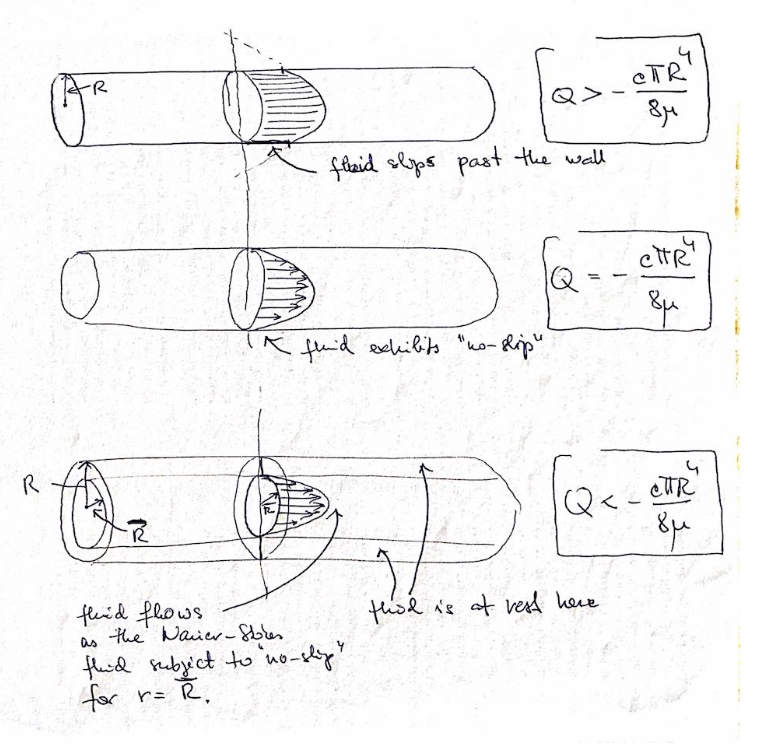
\includegraphics{Screenshot 2023-08-24 141914.png}
\end{figure}

\end{document}
